\pagebreak

\section{Introduction}
\label{sec:introduction}

% state the learning objective
\paragraph{} 
The objective of this laboratory assignment is to study and implement an Audio Amplifier circuit while, at the same time, trying to maximize the figure of merit M. The Audio Amplifier circuit can be separated into two stages: a Gain Stage, which can be simply described as the point in the system where the signal passes through an amplifier, and an Output stage. The role of the Output Stage is to provide power gain. It is also important to note that an Output Stage should have high input impedance and low output impedance. The circuit can be seen in Figure~\ref{fig:circuit}.


The implementation of the Audio Amplifier circuit was made according to the theoretical or simulation principles we were based on, using the equations presented in the class slides as the main material source to be able to do this fourth laboratory assignment.



\paragraph{}
In Section~\ref{sec:theoretical}, a theoretical introduction is made in order to contextualize all the main principles that sustain our construction and analysis of the circuit. A theoretical Audio Amplifier circuit is built and carefully analysed in Section~\ref{sec:analysis}, where the results are obtained in GNU Octave. Also, in Section~\ref{sec:simulation}, the Audio Amplifier circuit is analysed by simulation through the use of NGSpice to simulate the real electric circuit behaviour. The results of the simulation of Section~\ref{sec:simulation} are then compared to the theoretical results obtained in Section~\ref{sec:analysis} and the comparative results are expressed in Section~\ref{sec:erroranalysis}. The figure of merit, calculated according to the components used to build the simulation circuit, can also be found in Section~\ref{sec:erroranalysis}. The conclusions of this study are outlined in the final part of the report, in Section~\ref{sec:conclusion}.


\begin{figure}[h] \centering
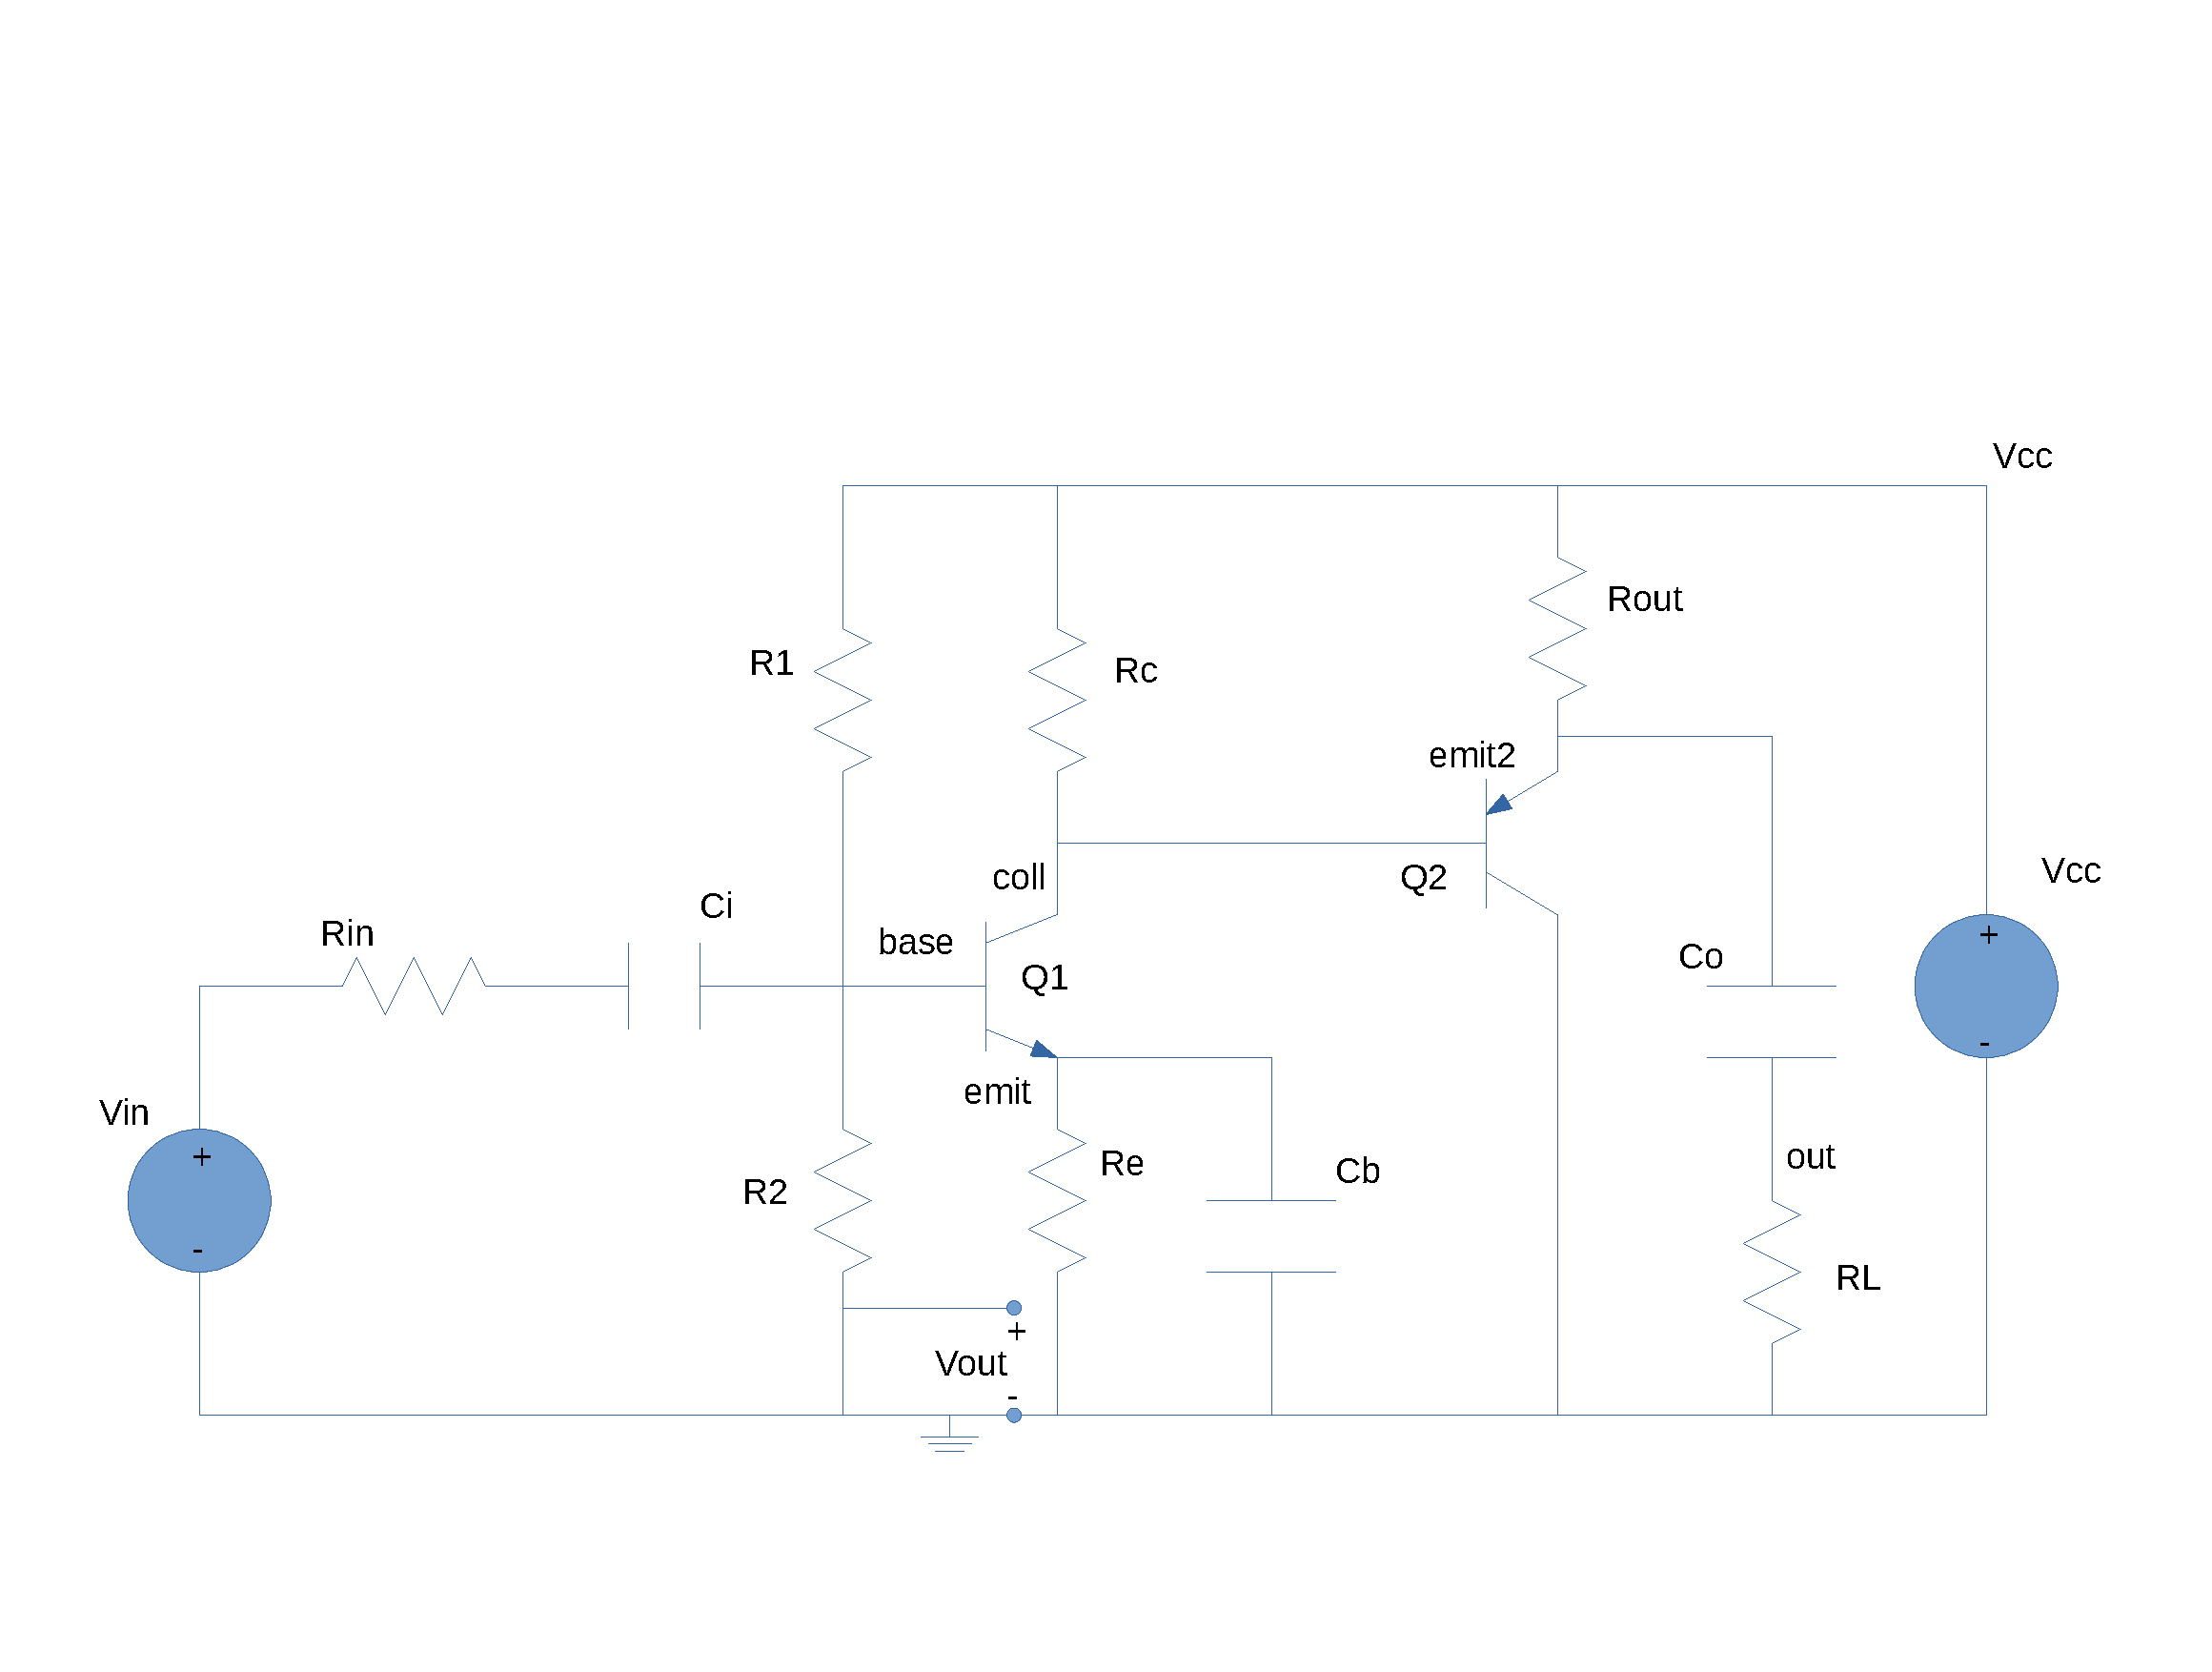
\includegraphics[width=0.8\linewidth]{circuit.pdf}
\caption{Fourth laboratory circuit.}
\label{fig:circuit}
\end{figure}

\pagebreak

